% !TeX spellcheck = <none>

\documentclass[a4paper,12pt]{report}

\usepackage{color}
\usepackage{xparse}
\usepackage{fourier}
\usepackage{amsmath}
\usepackage{dirtree}
\usepackage{verbatim}
\usepackage{fancyhdr}
\usepackage{graphicx}
\usepackage{outlines}
\usepackage{enumitem}
\usepackage{geometry}
\usepackage{fancyvrb}
\usepackage{listings}
\usepackage{multicol}
\usepackage{makecell}
\usepackage{setspace}
\usepackage{subcaption}
\usepackage{transparent}
\usepackage{indentfirst}
\usepackage{transparent}
\usepackage[usenames,dvipsnames,table]{xcolor}
\usepackage{datenumber,fp}
\usepackage{lstautogobble}
\usepackage[none]{hyphenat}
\usepackage[explicit]{titlesec}
\usepackage[breakable]{tcolorbox}
\usepackage[font=footnotesize]{caption}
\usepackage[colorlinks,linkcolor=blue,citecolor=red,urlcolor=gray]{hyperref}
\tcbuselibrary{breakable, skins}
\usepackage{fontspec}
\usepackage{fontawesome}

%% ------------ font settings -------------
\setmainfont{Consolas}

%% ----------- helper command -------------

\newcommand{\lrm}[1]{\textcolor{steelBlue}{\texttt{#1}}}
\newcommand{\qt}[1]{``#1''}

\definecolor{ao}				{rgb}{0.00, 0.50, 0.00}
\definecolor{codeGreen}			{rgb}{0.00, 0.70, 0.50}
\definecolor{lavendergray}		{rgb}{0.87, 0.86, 0.92}
\definecolor{mint}				{rgb}{0.24, 0.71, 0.54}
\definecolor{aliceblue}			{rgb}{0.94, 0.97, 1.00}
\definecolor{customCommentGreen}{rgb}{0.13, 0.65, 0.47}
\definecolor{steelBlue}			{rgb}{0.00, 0.00, 0.50}
\definecolor{blueLink}			{rgb}{0.10, 0.05, 0.67}
\definecolor{stringGreen}		{rgb}{0.00, 0.50, 0.00}

\definecolor{edge}				{rgb}{0.00, 0.45, 0.82}
\definecolor{twitter}			{rgb}{0.11, 0.63, 0.95}
\definecolor{linkedin}			{rgb}{0.00, 0.47, 0.71}
\definecolor{telegram}			{rgb}{0.15, 0.62, 0.85}
\definecolor{gmail}				{rgb}{0.87, 0.33, 0.28}

\DeclareCaptionFormat{listing}{\vskip1pt#1#2#3}
\captionsetup[lstlisting]{format=listing,singlelinecheck=false, margin=0pt, font={sf},labelsep=space,labelfont ={sf}}
\renewcommand\lstlistingname{snippet code}

\setlength{\headheight}{12pt}

\fancypagestyle{plain}{%
	\fancyhf{}%
	\renewcommand{\headrulewidth}{0pt}%
	\rhead{
		{\hypersetup{urlcolor=black}\hyperref{https://github.com/SMR76}{}{}{\faGithub}}
		{\hypersetup{urlcolor=twitter}\hyperref{https://twitter.com/S\_M\_R\_67}{}{}{\faTwitter}}
		{\hypersetup{urlcolor=linkedin}\hyperref{https://www.linkedin.com/in/seyyed-morteza-razavi-403b2a196/}{}{}{\faLinkedin}}
		{\hypersetup{urlcolor=Magenta}\hyperref{https://www.instagram.com/s\_m\_r76/}{}{}{\faInstagram}}
		{\hypersetup{urlcolor=telegram}\hyperref{tg://resolve?domain=S\_M\_R0}{}{}{\faSendO}}
		{\hypersetup{urlcolor=gmail}\hyperref{mailto:seyyed.morteza.razavi.76@gmail.com}{}{}{\faAt}}
	}
}

\pagestyle{plain}


% xepersian configuration.
\usepackage{xepersian}

\settextfont{Vazir}
\setlatintextfont{Carlito}

\rfoot{
	\footnotesize \today \\
	\lr{\href{https://github.com/SMR76/curriculum-vitae/raw/main/cv.en.pdf}{En}, Fa} \\
}

\begin{document}
	\lstset{
		frame=tb,
		basicstyle=\color{steelBlue}\linespread{0.8}\ttfamily,
		columns=fullflexible,
		keepspaces=false,
		tabsize=4,
		autogobble,
		breaklines=true,
		breakatwhitespace=true,
		stringstyle=\color{orange},
		commentstyle=\color{gray},
		keywordstyle=\color{purple},
		language=java,
		aboveskip=3mm,
		belowskip=3mm,
		showstringspaces=false,
		columns=flexible,
		captionpos=b,
		numbers=left,
		numbersep=5pt,
		numberstyle=\color{gray}\linespread{0.8}\ttfamily,
		postbreak=\mbox{\textcolor{blue}{$\hookrightarrow$}\space}
	}

	\newcounter{dateone}%
	\newcounter{datetwo}%
	\setmydatenumber{dateone}{1997}{11}{25}%
	\setmydatenumber{datetwo}{\the\year}{\the\month}{\the\day}%
	\FPeval\myage{trunc(div(sub(\thedatetwo,\thedateone),365.2425),0)}

	\noindent
	\begin{center}


	\textbf{رزومه}
	\noindent\textcolor{gray}{\rule{\linewidth}{0.5pt}}
	\textit{
	مرتضیٰ رضوی هستم}\\
	\textit{
	برنامه‌نویس
	\lr{C++} و \lr{QML}.}\\[8mm]
	سن:
	\myage\smallskip\\
	کارشناسی کامپیوتر دانشگاه
	\href{https://en.wikipedia.org/wiki/Quchan\_University\_of\_Advanced\_Technologies\_Engineering}
	{قوچان}\\
	\noindent\textcolor{gray}{\rule{\linewidth}{0.5pt}}
	برنامه‌های نوشته شده توسط بنده.\\
	\textsubscript{تم‌ها}\\
	شامل چندین
	\lr{Style}
	برای
	\lr{Component}%
	های
	\lr{QtQuick}.
	\begin{latin}
		\centering
		\href{https://github.com/SMR76/qml-neumorphism}{Neumorphism},
		\href{https://github.com/SMR76/qml-snow-white}{Snow White},
		\href{https://github.com/SMR76/qooey}{Qooey},
		\href{https://github.com/SMR76/qube}{Qube},
		\href{https://github.com/SMR76/glitch}{Glitch},
		\href{https://github.com/SMR76/hive}{Hive}
	\end{latin}
	\vspace{5mm}
	\textsubscript{برنامه‌ها}
	\begin{latin}
		\href{https://github.com/SMR76/knight-pen}{Knight Pen},
		\href{https://github.com/SMR76/cardian}{Qloudy},
		\href{https://github.com/SMR76/cardian}{Cardian}
	\end{latin}
	\textsubscript{ابزارها}
	\begin{latin}
		\centering
		\href{https://github.com/SMR76/icon-manager}{Icon Manager},
		\href{https://github.com/SMR76/qomponent}{Qomponent}
	\end{latin}
	\vspace{5mm}
	\textsubscript{وب}
	\begin{latin}
		\centering
		\href{https://smr76.github.io}{smr76.github.io},
		\href{https://github.com/SMR76/smr-wp-plugin}{Wordpress Plugin}
	\end{latin}
	\vspace{5mm}
	\textsubscript{طراحی‌ها}\\
	\href{https://www.instagram.com/one.red.little.fish}{\lr{instagram}}
	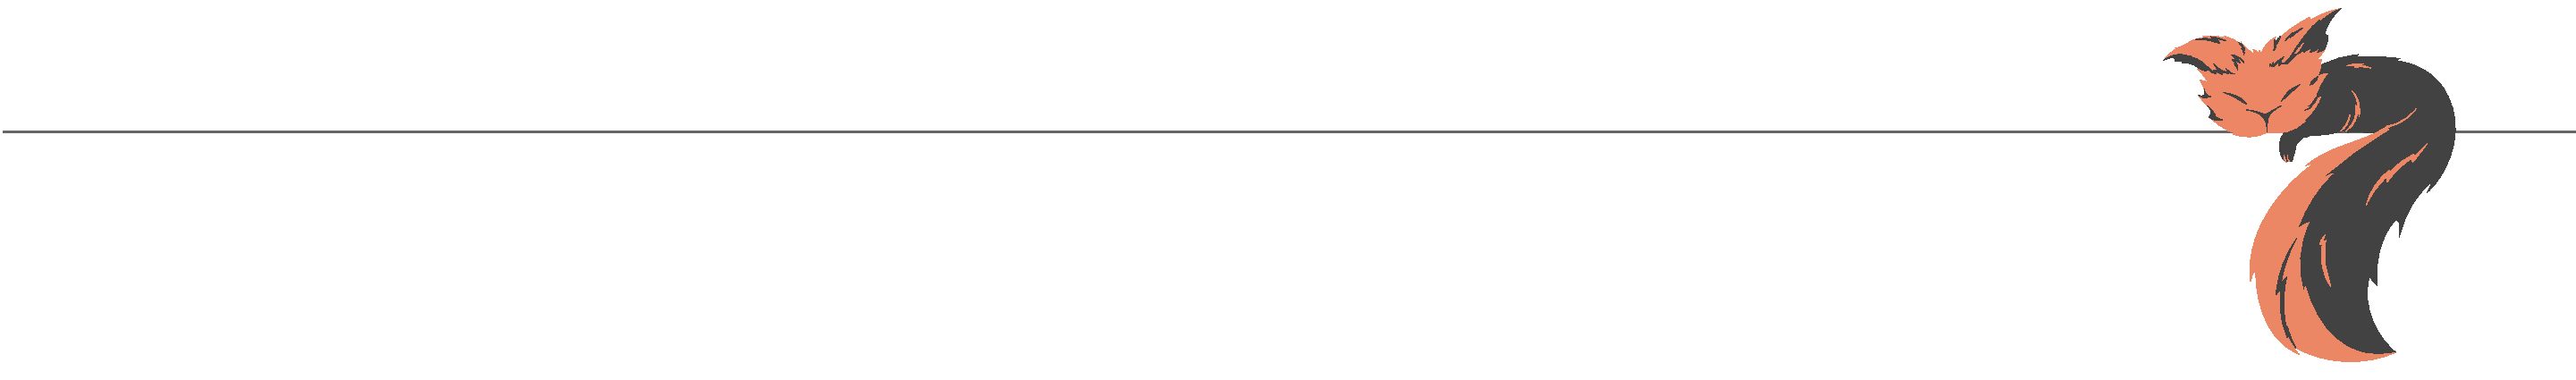
\includegraphics[width=\linewidth]{./sleeping-fox.pdf}\vspace*{-10mm}
	تماس با من
	\end{center}
	\begin{itemize}[nosep]
		\item \textcolor{gmail}{\faAt}
		پست الکترونیک:
		\href{mailto:seyyed.morteza.razavi.76@gmail.com} {\lr{seyyed.morteza.razavi.76@gmail.com}}
		\item \textcolor{telegram}{\faSendO}
		تلگرام:
		\href{https://s\_m\_r0.t.me}{\lr{@S\_M\_R0}}
		\item \textcolor{edge}{\faEdge}
		وبسایت:
		\href{https://SMR76.github.io/#contactMe}{\lr{smr76.github.io}}
	\end{itemize}
\end{document}
